    
\section{Exploratory Analysis}

    %data was preprocessed as described in methods

    \subsection{Main effect subgroups}

    There are three main effects by which breast cancer samples can be stratified into groups: morphology, stage and PAM50 molecular profile. PCA is able separate samples into tumour/normal sample clusters fairly well (shown as an example in Methods, Figure \ref{fig:pcamethod}. However, it is more interesting to apply PCA to explore variation coming from separating samples in different cancer classification groups.  
    
    PCA was applied to 969 samples (857T, 112N), which were divided into subgroups by three systematic effect groups (i.e. PAM50, tumour morphology, cancer stage), which subgroup sizes shown in Tables \ref{table:morphstage} and \ref{table:pam50counts}. \\
    Figure \ref{fig:pcapam50} shows the PCA plot of first two principal components, coloured by PAM50 molecular subtype groups. PC1 accounts for 11\% of the total variation in the data, and is driven by the differences between normal and cancer samples. PC2 accounts for 8.6\% of the variation, and characterises the variation among breast cancer subtypes. Firstly, Basal-like samples form a separate cluster (orange), which emphasises its complete dissimilarity at molecular level. Luminal A and Luminal B form a partially overlapping cluster (yellow and red), which is expected from the known similarities of these subtypes. HER2-enriched cluster (blue) is understandably located between Luminal B and Basal-like as it is known to share expression profiles with these two. And lastly, seeing Normal-like subtype (pink) overlapping with normal samples (green) as well as with Luminal A cancer subtype fits nicely with the fact that Normal-like subtype shares morphology with the former and IHC and molecular profile with the latter.    
    
    % PAM50 PCA plot 
            \begin{figure}[!h]
            \centering
            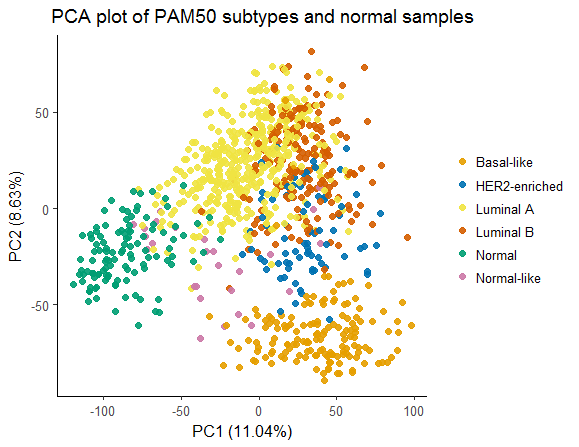
\includegraphics[scale=0.37]{pcapam502.png} 
            \caption{PCA plot showing the variance along PC1 and PC2 for PAM50 molecular subtypes of breast cancer and normal samples}
            \label{fig:pcapam50}
            \end{figure}
            
    \newpage
    Figure \ref{fig:1dpcapam50} shows the results of PCA for the first nine PCs, as described in the Methods section. Looking at the results in this way highlights again that PC1 is driven by tumour/normal variation. Together with PC2 they also capture the differences among PAM50 subtypes. As the PCs numbers increase, variation captured by them decreases. 
    
    % PAM50 1d PCA plot 
            \begin{figure}[!h]
            \centering
            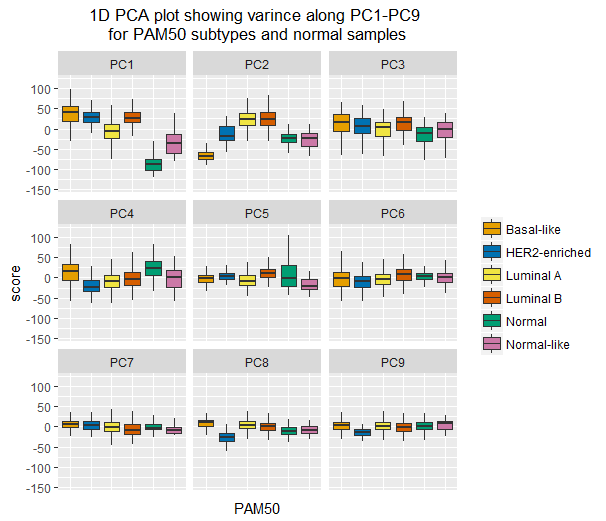
\includegraphics[scale=0.5]{1dpcapam50.png}
            \caption{One-dimensional PCA plots showing variance along PC1-PC9 for PAM50 molecular subtypes of breast cancer and normal samples. }
            \label{fig:1dpcapam50}
            \end{figure}
    
    
    The PCA results for morphology and stages classifications are shown in Figure \ref{fig:1dpcamorphstage} as one-dimensional variation plots. It can be observed that PCA was not able to capture as much variation between morphology groups and stages as among PAM50 subtypes. From one-dimensional plots it is evident that PC1 captures cancer/normal differences in both classification types. However, the rest of PCs do not capture enough variation to be evident on 2D PCA plots, therefore here only 1D plots are presented. Appendix \ref{} show 2D plots for results completion.    
    
    % 1D PCA for stages and morphology
            
            \begin{figure}[!h]
            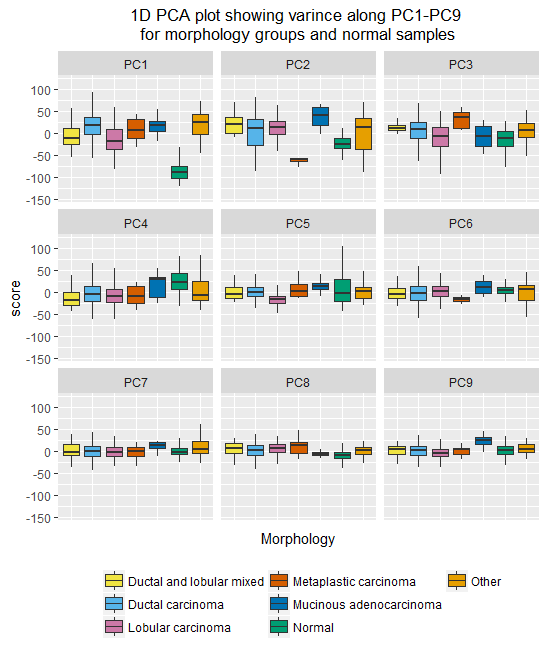
\includegraphics[width=0.4\linewidth]{1dpcamorph2.png}\hfill
            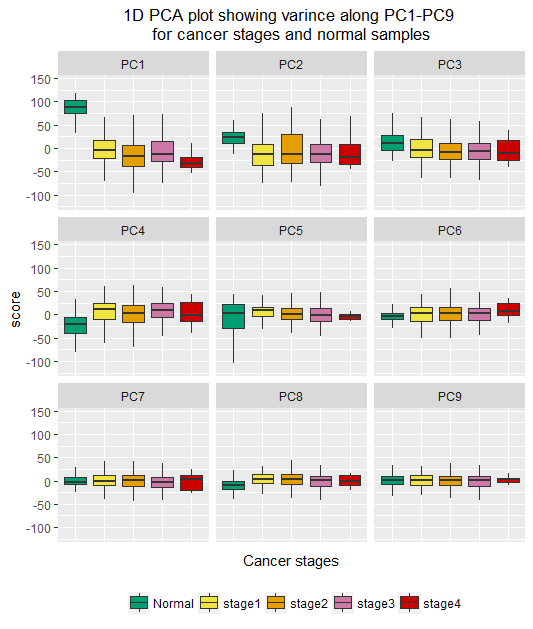
\includegraphics[width=0.4\linewidth]{1dpcastages2.png}
            \caption{One-dimensional PCA plots showing variance along PC1-PC9 for morphology groups and stages, with normal samples.}
            \label{fig:1dpcamorphstage}
            \end{figure}
            
    
    \newpage
    Interestingly, PCA was not able to capture any significant differences between stages (e.g. stage 1 and stage 4), where the differences in expression should be evident and therefore reflected in PCA results. The same is the case for two main distinct mythologies - Lobular and Ductal carcinomas, which overlap greatly. A possible explanation for these results is the unbalanced sizes of subgroups in these two classification methods, as well as their composition in terms of PAM50 subtypes, which is evidently the main driving force in sample classifications. 
    
    To explore this idea, the sample count data was visualised as stacked barplots presented in Figure \ref{fig:barms}. Each bar shows the total count of samples of a chosen morphology (left plot) or stage (right plot). The differing group sizes are evident.         
    
    % barsplots for stages and morphology 
       
        \begin{figure}[!h]
        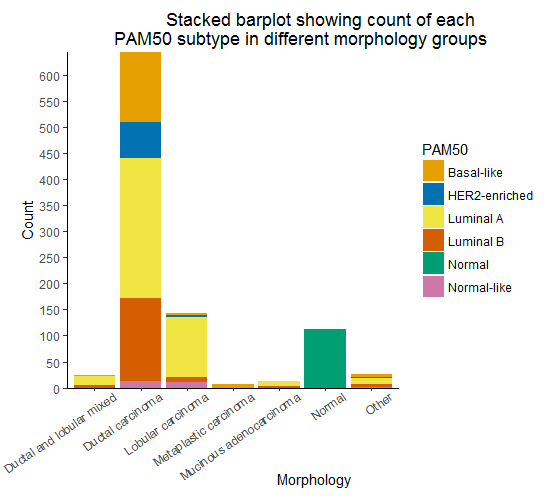
\includegraphics[width=0.53\linewidth]{bar_morph.png}\hfill
        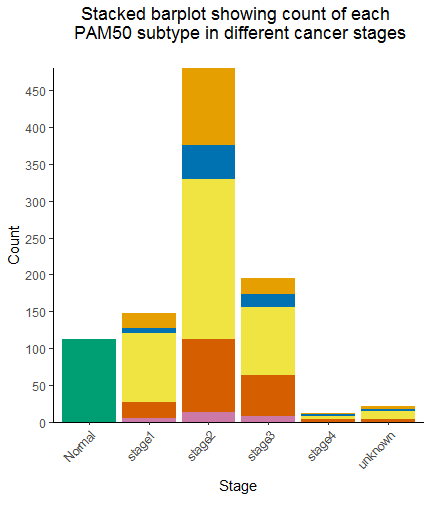
\includegraphics[width=0.4\linewidth]{bar_stages2.png}
        \caption{Stacked barplots of sample number counts per subgroups in morphology groups and stages classification groups. The coloured proportions represent PAM50 subtypes samples within each subgroup.}
        \label{fig:barms}
        \end{figure}
        
    Ductal carcinoma morphology samples make up over 70\% of all samples (x/857), but are well-proportionate in terms of PAM50 composition (i.e. similar proportions as the full dataset, with Luminal A dominating). Other subgroups, however, in addition to being smaller, are restricted to only a few PAM50 subtypes. For instance, Metaplastic carcinoma is made up completely of Basal-like samples, while Mucinous morphology is represented by only Luminal subtypes (the counts are shown in Table \ref{table:counts}). This observation explains why these two mophologies are separated in 1D PCA plot in PC2 (Figure \ref{fig:1dpcamorphstage}) - the difference between Luminal and Basal tissues is driving this variation. However, it is important to note, that there is a chance that these two morphologies, Metaplastic and Mucinous, actually only exists as Basal and Luminal subtype, respectively, but it is not possible to claim for or against this based on the current dataset.    
    
    The sample count difference between stages are also noticeable, which stage 2 accounting for roughly 50\% of the samples. The proportions of PAM50 subtypes within stages 1-3 appear to be well-balanced. Stage 4 is, however, of major concern. It has an alarmingly low sample count and is not represented in Normal-like subtype. The counts are shown in Table \ref{table:counts}.
        
        
    %TABLE x3 counts   
                \begin{table}[!h]
                \centering
                \caption{Samples number counts in pairwise comparisons of three main breast cancer samples classifications. Top table: PAM50 and stages, Middle table: PAM50 and morphology, Bottom table: stages and morphology. Each table shows row and column sums for each subgroup. The total count of samples in the project is in the lower right corner: 857.}
                \label{table:counts}
                \resizebox{\textwidth}{!}{%
                \begin{tabular}{ccccccc}
                \small
                \multicolumn{1}{l|}{} & \multicolumn{1}{c|}{\textbf{Luminal A}} & \multicolumn{1}{c|}{\textbf{Luminal B}} & \multicolumn{1}{c|}{\textbf{Basal-like}} & \multicolumn{1}{c|}{\textbf{HER2-enriched}} & \multicolumn{1}{c|}{\textbf{Normal-like}} & {\color[HTML]{9B9B9B} \textit{rowsums}} \\ \hline
                \multicolumn{1}{c|}{\textbf{stage 1}} & \multicolumn{1}{c|}{94} & \multicolumn{1}{c|}{22} & \multicolumn{1}{c|}{21} & \multicolumn{1}{c|}{6} & \multicolumn{1}{c|}{5} & \multicolumn{1}{c|}{{\color[HTML]{656565} 148}} \\ \hline
                \multicolumn{1}{c|}{\textbf{stage 2}} & \multicolumn{1}{c|}{217} & \multicolumn{1}{c|}{99} & \multicolumn{1}{c|}{105} & \multicolumn{1}{c|}{47} & \multicolumn{1}{c|}{13} & \multicolumn{1}{c|}{{\color[HTML]{656565} 481}} \\ \hline
                \multicolumn{1}{c|}{\textbf{stage 3}} & \multicolumn{1}{c|}{93} & \multicolumn{1}{c|}{55} & \multicolumn{1}{c|}{21} & \multicolumn{1}{c|}{18} & \multicolumn{1}{c|}{8} & \multicolumn{1}{c|}{{\color[HTML]{656565} 195}} \\ \hline
                \multicolumn{1}{c|}{\textbf{stage 4}} & \multicolumn{1}{c|}{4} & \multicolumn{1}{c|}{4} & \multicolumn{1}{c|}{2} & \multicolumn{1}{c|}{2} & \multicolumn{1}{c|}{{\color[HTML]{C0C0C0} x}} & \multicolumn{1}{c|}{{\color[HTML]{656565} 12}} \\ \hline
                \multicolumn{1}{c|}{\textbf{unknown}} & \multicolumn{1}{c|}{12} & \multicolumn{1}{c|}{3} & \multicolumn{1}{c|}{4} & \multicolumn{1}{c|}{2} & \multicolumn{1}{c|}{{\color[HTML]{C0C0C0} x}} & \multicolumn{1}{c|}{{\color[HTML]{656565} 21}} \\ \hline
                \multicolumn{1}{c|}{{\color[HTML]{9B9B9B} \textit{colsums}}} & \multicolumn{1}{c|}{{\color[HTML]{656565} 420}} & \multicolumn{1}{c|}{{\color[HTML]{656565} 183}} & \multicolumn{1}{c|}{{\color[HTML]{656565} 153}} & \multicolumn{1}{c|}{{\color[HTML]{656565} 75}} & \multicolumn{1}{c|}{{\color[HTML]{656565} 26}} & \multicolumn{1}{c|}{\textit{857}} \\ \cline{2-7} 
                \multicolumn{1}{l}{} & \multicolumn{1}{l}{} & \multicolumn{1}{l}{} & \multicolumn{1}{l}{} & \multicolumn{1}{l}{} & \multicolumn{1}{l}{} & \multicolumn{1}{l}{} \\
                \multicolumn{1}{c|}{} & \multicolumn{1}{c|}{\textbf{Luminal A}} & \multicolumn{1}{c|}{\textbf{Luminal B}} & \multicolumn{1}{c|}{\textbf{Basal-like}} & \multicolumn{1}{c|}{\textbf{HER2-enriched}} & \multicolumn{1}{c|}{\textbf{Normal-like}} & {\color[HTML]{9B9B9B} \textit{rowsums}} \\ \hline
                \multicolumn{1}{c|}{\textbf{Lobular}} & \multicolumn{1}{c|}{114} & \multicolumn{1}{c|}{10} & \multicolumn{1}{c|}{3} & \multicolumn{1}{c|}{5} & \multicolumn{1}{c|}{11} & \multicolumn{1}{c|}{{\color[HTML]{656565} 143}} \\ \hline
                \multicolumn{1}{c|}{\textbf{Ductal}} & \multicolumn{1}{c|}{270} & \multicolumn{1}{c|}{158} & \multicolumn{1}{c|}{135} & \multicolumn{1}{c|}{68} & \multicolumn{1}{c|}{13} & \multicolumn{1}{c|}{{\color[HTML]{656565} 644}} \\ \hline
                \multicolumn{1}{c|}{{\color[HTML]{000000} \textbf{LobDuctal}}} & \multicolumn{1}{c|}{17} & \multicolumn{1}{c|}{6} & \multicolumn{1}{c|}{1} & \multicolumn{1}{c|}{{\color[HTML]{C0C0C0} x}} & \multicolumn{1}{c|}{{\color[HTML]{C0C0C0} x}} & \multicolumn{1}{c|}{{\color[HTML]{656565} 24}} \\ \hline
                \multicolumn{1}{c|}{\textbf{Metaplastic}} & \multicolumn{1}{c|}{{\color[HTML]{C0C0C0} x}} & \multicolumn{1}{c|}{{\color[HTML]{C0C0C0} x}} & \multicolumn{1}{c|}{7} & \multicolumn{1}{c|}{{\color[HTML]{C0C0C0} x}} & \multicolumn{1}{c|}{{\color[HTML]{C0C0C0} x}} & \multicolumn{1}{c|}{{\color[HTML]{656565} 7}} \\ \hline
                \multicolumn{1}{c|}{\textbf{Mucinous}} & \multicolumn{1}{c|}{8} & \multicolumn{1}{c|}{4} & \multicolumn{1}{c|}{{\color[HTML]{C0C0C0} x}} & \multicolumn{1}{c|}{{\color[HTML]{C0C0C0} x}} & \multicolumn{1}{c|}{{\color[HTML]{C0C0C0} x}} & \multicolumn{1}{c|}{{\color[HTML]{656565} 12}} \\ \hline
                \multicolumn{1}{c|}{\textbf{Other}} & \multicolumn{1}{c|}{11} & \multicolumn{1}{c|}{5} & \multicolumn{1}{c|}{7} & \multicolumn{1}{c|}{2} & \multicolumn{1}{c|}{2} & \multicolumn{1}{c|}{{\color[HTML]{656565} 27}} \\ \hline
                \multicolumn{1}{c|}{{\color[HTML]{9B9B9B} \textit{colsums}}} & \multicolumn{1}{c|}{{\color[HTML]{656565} 420}} & \multicolumn{1}{c|}{{\color[HTML]{656565} 183}} & \multicolumn{1}{c|}{{\color[HTML]{656565} 153}} & \multicolumn{1}{c|}{{\color[HTML]{656565} 75}} & \multicolumn{1}{c|}{{\color[HTML]{656565} 26}} & \multicolumn{1}{c|}{\textit{857}} \\ \cline{2-7} 
                \multicolumn{1}{l}{} & \multicolumn{1}{l}{} & \multicolumn{1}{l}{} & \multicolumn{1}{l}{} & \multicolumn{1}{l}{} & \multicolumn{1}{l}{} & \multicolumn{1}{l}{} \\
                \multicolumn{1}{c|}{} & \multicolumn{1}{c|}{\textbf{stage 1}} & \multicolumn{1}{c|}{\textbf{stage 2}} & \multicolumn{1}{c|}{\textbf{stage 3}} & \multicolumn{1}{c|}{\textbf{stage 4}} & \multicolumn{1}{c|}{\textbf{unknown}} & {\color[HTML]{9B9B9B} \textit{rowsums}} \\ \hline
                \multicolumn{1}{c|}{\textbf{Lobular}} & \multicolumn{1}{c|}{14} & \multicolumn{1}{c|}{78} & \multicolumn{1}{c|}{49} & \multicolumn{1}{c|}{{\color[HTML]{C0C0C0} x}} & \multicolumn{1}{c|}{2} & \multicolumn{1}{c|}{143} \\ \hline
                \multicolumn{1}{c|}{\textbf{Ductal}} & \multicolumn{1}{c|}{118} & \multicolumn{1}{c|}{368} & \multicolumn{1}{c|}{129} & \multicolumn{1}{c|}{11} & \multicolumn{1}{c|}{18} & \multicolumn{1}{c|}{644} \\ \hline
                \multicolumn{1}{c|}{\textbf{LobDuctal}} & \multicolumn{1}{c|}{5} & \multicolumn{1}{c|}{11} & \multicolumn{1}{c|}{7} & \multicolumn{1}{c|}{{\color[HTML]{C0C0C0} x}} & \multicolumn{1}{c|}{1} & \multicolumn{1}{c|}{644} \\ \hline
                \multicolumn{1}{c|}{\textbf{Metaplastic}} & \multicolumn{1}{c|}{5} & \multicolumn{1}{c|}{11} & \multicolumn{1}{c|}{7} & \multicolumn{1}{c|}{{\color[HTML]{C0C0C0} x}} & \multicolumn{1}{c|}{1} & \multicolumn{1}{c|}{24} \\ \hline
                \multicolumn{1}{c|}{\textbf{Mucinous}} & \multicolumn{1}{c|}{2} & \multicolumn{1}{c|}{4} & \multicolumn{1}{c|}{1} & \multicolumn{1}{c|}{{\color[HTML]{C0C0C0} x}} & \multicolumn{1}{c|}{{\color[HTML]{C0C0C0} x}} & \multicolumn{1}{c|}{7} \\ \hline
                \multicolumn{1}{c|}{\textbf{Other}} & \multicolumn{1}{c|}{6} & \multicolumn{1}{c|}{15} & \multicolumn{1}{c|}{5} & \multicolumn{1}{c|}{1} & \multicolumn{1}{c|}{{\color[HTML]{C0C0C0} x}} & \multicolumn{1}{c|}{27} \\ \hline
                \multicolumn{1}{c|}{{\color[HTML]{9B9B9B} \textit{colsums}}} & \multicolumn{1}{c|}{148} & \multicolumn{1}{c|}{481} & \multicolumn{1}{c|}{195} & \multicolumn{1}{c|}{12} & \multicolumn{1}{c|}{21} & \multicolumn{1}{c|}{\textit{857}} \\ \cline{2-7} 
                \end{tabular}%
                }
                \end{table}

        
        
    \newpage  
    
    Another way of exploring the structure within a dataset and the relevance of different classification conventions is to perform sample clustering and visualise it as a heatmap. Figure \ref{fig:heatmap1k} shows the results of performing clustering on top 1000 highest variance genes. Variance was computed for each row (gene) in cancer samples only, and the top 1000 were selected to be used for clustering, as the genes with the most differences are of interest. The three main effect groups are shown above the heatmap as colour bars, which enables side-by-side comparisons.     
    
    % heatmap 1000
            \begin{figure}[!h]
            \centering
            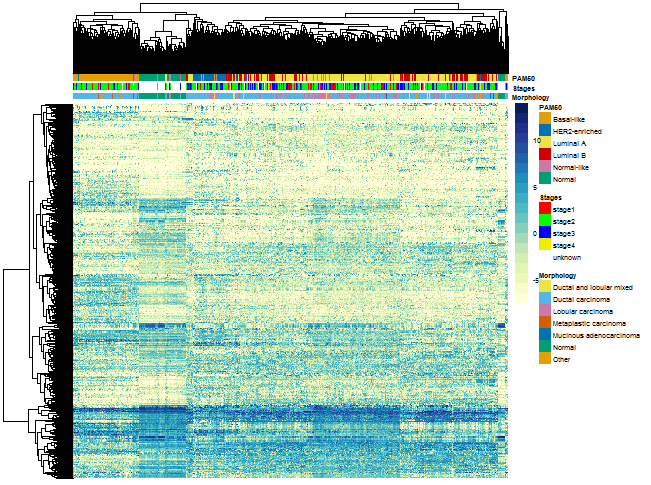
\includegraphics[scale=0.8]{heatmap_top1k.png}
            \caption{Heatmap with clustering on top 1000 highest variance genes (calculated on cancer samples only). The data is clustered by columns (samples) and rows (genes), with dendograms showing how clusters are formed. The colour bars above the heatmap (PAM50, stages, morphology) show the subgroups to which each sample belongs, colour-coded according to the legend on the right. The colours of heatmap represent gene expression intensity according to the scale (high expression - dark blue, low expression - light yellow). The data was clustered with Euclidean distance and average linkage. }
            \label{fig:heatmap1k}
            \end{figure}
    
    First and foremost, the unsupervised clustering was able to form two main clusters: Luminal and non-Luminal samples. Cluster on the right contains the majority of Luminal A and Luminal B samples according to the top colour bar (PAM50). The left hand side cluster contains Basal-like, HER2-enriched, and normal samples. Normal-like subtype is scattered across the entire dendogram, with more notable appearance inbetween Luminal A and normal samples, as expected. The Basal-like cluster is well-defined, which highlights this subtype difference from the rest. The Luminal types are mixed as anticipated. Overall, clustering is in line with the PCA results for PAM50 subtypes. \\
    With regards to stages and morphology colour bars, it can be observed that clustering, much like PCA, was not able to find any distinct major patterns among their subgroups. Again, the sizes of the subgroups may partially be responsible for that. It is a challenge to spot the minority-sized subgroups on the colour bar, and very clear to see how Ductal carcinoma dominates the dataset (light blue, third bar). The colour bar of stages also shows no distinct patterns. 
    
    \newpage
    However, another idea worth investigation is to test how data will cluster if sub-subgroups averages are taken. As stages of cancer progression are of high interest in this project, the averages of each PAM50 subtype at each stage were taken and clustered. Figure \ref{fig:dendogram} shows the resulting dendogram. 
    
        % dendogram
            \begin{figure}[!h]
            \centering
            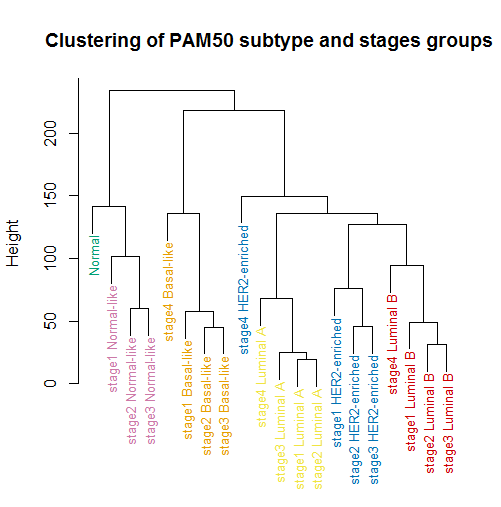
\includegraphics[scale=0.45]{dendogram2.png}
            \caption{Dendogram showing clustering of PAM50 subtypes within stages (averages per stage per subtypes)}
            \label{fig:dendogram}
            \end{figure}
    
    Remarkably, all subtypes form distinct branch clusters (expect HER2-enriched). Normal and Normal-like samples are the outgroup, understandably, and then Basal-like subtype is also an outgroup to the rest of samples. Luminal types and HER2-enriched are separated to well-defined branches. It is important to note that each subtype cluster has stage 4 branch as an outgroup, with the exception of HER2-enriched stage4, which is only made up of 2 samples perhaps leading to an unstable average. Seeing stage 4 as an outgroup is an important observation, as it is the most different and severe (due to metastasis) stage of cancer progression. \\
    
    Lastly, seeing the samples cluster primarily by PAM50 and only then by stage in Figure \ref{fig:dendogram}, is yet another evidence to what was observed with PCA and heatmap clustering. PAM50 is the main classification effect of breast cancer samples. When using other classification methods, PAM50 subtypes have to be taken into account. For example, comparing two morphologies might now produce expected results if their PAM50 subtype sample composition will be the main driving effect of differences. So the heterogeneity of groups has to be taken into account, and the downstream analysis has to be done on sub-subgroups.  
    
 
   

    

    
 
    
    \newpage
     \subsubsection{Cofactors and batch effects}
    The metadata available for each sample was explored with PCA to check for sources of unusual variation.
    
    The potential batch effect groups are the year the sample was taken from the patient (i.e. lab protocol standards have changed over the years), as well as the actual source site (i.e. where the sample was taken and processed). Additionally, patient age groups were explored. 
    
    One-dimensional PCA plots were used to visualise variation over the years and across the sites. 
    Figure \ref{} shows the first X PCs of PCA on the year data. Each boxplot represents samples taken in a single year. The boxplots are samples sequentially (as shown in the figure legend)
    
    
    %talk about variton in years.  protocls in introduced in 2005. 
    
    %sites
    
    %age groups
    


\section{Looking for Autophagy signatures}

    \subsection{Differential Expression Testing}
    
        \subsubsection{Enrichment Analysis}

    \subsection{Soft clustering}
    
        \subsubsection{Enrichment Analysis}
    
\section{Downstream}
